\documentclass[11pt]{article}
\usepackage[letterpaper,left=18mm,right=18mm,top=21mm,bottom=18mm,headheight=14pt,headsep=5mm]{geometry}
\usepackage[T1]{fontenc}
\usepackage{helvet}
\renewcommand{\familydefault}{\sfdefault}
\usepackage{amsmath,amssymb,array,tabularx,booktabs,tikz,fancyhdr}
\usetikzlibrary{arrows.meta}
\usepackage[hidelinks]{hyperref}
\pagestyle{fancy}\fancyhf{}
\fancyhead[L]{\small Week 55 / Few sums and equal spacing / Facilitator}
\fancyfoot[L]{\footnotesize Bellingham Math Circle / Week 55 / W55-F-v1}
\fancyfoot[R]{\footnotesize\thepage}
\renewcommand{\headrulewidth}{0.4pt}
\setlength{\parindent}{0pt}\setlength{\parskip}{6pt}
\setlength{\tabcolsep}{5pt}\renewcommand{\arraystretch}{1.18}
\hyphenpenalty=7000\exhyphenpenalty=7000
\pdfinfoomitdate=1\pdftrailerid{}
\newcommand{\heading}[1]{\vspace{4pt}{\large\bfseries #1}\par}
\newcommand{\sub}[1]{\textbf{#1}\par}
\newcommand{\sset}[1]{\{#1\}}
\newcommand{\smalltable}{\small\renewcommand{\arraystretch}{1.2}}
\begin{document}
\heading{Mathematical overview: sharp bounds and their equality case}
For \textbf{nonempty finite sets of integers} $A,B$, let $m=|A|$, $n=|B|$, and
\[
 A+B=\sset{a+b:a\in A,\ b\in B}.
 \qquad m+n-1\ \leq\ |A+B|\ \leq\ mn.
\]
Count \textbf{different values}, once each. There may be $mn$ ways to choose a pair but fewer different totals. Inputs contain different values within each set; the same value may occur in both inputs. Zero is a genuine card. Addition is ordinary integer addition, with \textbf{no wrapping}.

\textbf{Sharp minimum theorem.} If $m,n\geq2$, then $|A+B|=m+n-1$ if and only if both inputs are arithmetic progressions with the \textbf{same positive value gap} $d$. Their starting values and lengths may differ. Numerical gaps are differences of neighboring values in increasing order, not distances between printed cards.

\textbf{Singleton exception.} If $A=\sset{a}$, adding $a$ translates every member of $B$ without merging any two. Thus $|A+B|=|B|$ for \emph{every} nonempty $B$, including unevenly spaced inputs. The same holds with A and B exchanged. Empty inputs are excluded from the bound; duplicate cards are not additional set elements. The ordered bound need not hold modulo a number.

\textbf{Proof map.} Sort A upward and B rightward in an addition array. Any full right/up path has $m+n-1$ strictly increasing entries, proving the lower bound. The $mn$ pairs prove the upper bound. At lower equality, every full path contains the entire sumset. Swapping the route around any adjacent square forces its two alternative middle sums to agree, hence every A gap equals every B gap. Common-gap progressions attain the bound. Pages 7--8 give the complete argument; this is the exact extremal theorem, not the general Freiman theorem.

\sub{What children are meant to discover}
Different pairs can land on one total. Choosing the inputs changes how many such coincidences occur. Fewest totals suggest a rule for input sizes; common numerical gaps explain the sharp minimum. A one-card input reveals why the equality claim needs its two-card assumption. The grid supplies a certificate that no design can beat the lower bound.

\begin{tabularx}{\linewidth}{@{}p{29mm}X@{}}
\toprule
Entry / pages & Operational prerequisites and mathematical choices\\\midrule
Concrete core, 1--7 & Recognize 0--9 and add to 18, with occasional adult facts if needed; retain fixed inputs, merge repeated totals, choose new sets. Chiefly Grades 3--5; a ready second grader may enter. Adult reading is fine; children still choose and test.\\
Grid, 8 & Coordinate one row and one column, then follow right/up moves and distinguish moves from visited dots. Introduce only after concrete trials.\\
General, 9--10 & Interpret letters as card counts, use multiplication for pairs, reason beyond one example. The inverse proof needs two full paths and a local change. Readiness-dependent upper continuation, often with adult conversation.\\
K--1 & No independent sumset packet or K--1 coverage is claimed. A separate prior tiling option is specified on page 2.\\\bottomrule
\end{tabularx}
\newpage

\heading{Prepare for the fixed KK11 / 3333 / 445 tables}
\sub{Adults and kit counts}
The parent volunteer remains with the two kindergartners and two first graders. The second mathematician remains with the four third graders (two pairs). The organizer remains with the two fourth graders and fifth grader (one pair plus a checking referee; rotate roles). Keep the three tables fixed.

For \textbf{each active sumset pair}: two distinguishable decks 0--9, one labeled A and one B (20 cards); 20 counters, 8--10 mm diameter; pencil/eraser; blank paper or whiteboard; selected student pages. A third child checks the unchanged inputs and each pair's addition. Three active stations therefore need \textbf{60 number cards and 60 counters}, plus one spare deck pair if desired. Use A/B labels or different outlines as well as any color.

Make reusable cards from paper about 25$\times$35 mm, or use a suitable existing kit and label the decks. Lay the actual cards \textbf{beside} the sheet, in two clearly labeled lanes. Printed 13$\times$14 mm card outlines are pictures and places to write selected values; they are not card holders. Return unused cards to separate A/B piles. Keep the selected cards in place until a trial is saved. A zero card occupies a slot and participates like every other card.

\sub{Print and check the actual materials}
The student PDF is \textbf{ten US Letter landscape pages} (792$\times$612 pt), single-sided, at \textbf{100\% / Actual Size}. All headers say Grades 3--5. Each working result lane has 19 cells, labeled 0--18, of 12$\times$18 mm: total width 228 mm. A 10 mm counter has nominal 2 mm horizontal clearance; place it below the numeral. The page-8 9 mm grid dots are pencil diagrams, not counter spaces. Print this portrait adult guide separately. Do not scale the student sheets to fit a portrait page.

\textbf{First-visit print set:} three copies of student pages 1--3 (nine landscape sheets), one reserve copy of pages 4--10 (seven), and one selected K--1 board per child (four portrait sheets). Keep a joint marked record per station; give one page at a time. Parent uses the prior tiling guide; both mathematicians use this guide.

Before using the kit, measure one printed 12 mm cell; place and move the actual counters without obscuring labels; rehearse keeping cards fixed and saving marks before removing counters. Test whether a pair can check all pairs without losing its place. \textbf{Physical kit fit, material handling, launch rehearsal and classroom piloting have not been performed.} Digital dimensions do not establish these properties.

\sub{A separate K--1 option already in the collection}
Use a selected unfinished or unfamiliar board from the current Week 1 K--1 tiling packet, \texttt{week-01-k-1.pdf} (F01-K-v4), for example Problem 1's sailboat/cat or Problem 2's two fillings. This is an accepted prior activity option, not a new sumset entry. Ask the organizer/use log which boards were actually used; available pages do not establish prior completion. Print those boards at 100\% and match a small green triangle to the one-inch grid edge.

For four K--1 children, the existing guide's per-child allocation scales to \textbf{24 blue rhombi, 48 green triangles, 12 purple pieces}, and a few small red/yellow pieces per child; set larger Upscale pieces aside. The parent can trace a filling before pieces are reused. Use the existing Week 1 guide for solutions; its old roster/staffing paragraph is superseded by the fixed tables above.

\sub{An hour with flexible stopping points}
0--5 min: running/movement. 5--8: short material handling and shared demonstration. 8--25: concrete trials. 25--28: movement/reset. 28--52: continue or return to a different concrete question; offer a readiness-dependent bridge. 52--60: share one saved design, tidy, record what was actually used. These are proposed timings, not measured pacing.
\newpage

\heading{Launch, then let the concrete problem carry the work}
Let children handle cards and counters briefly. Bring everyone to the page-1 \textbf{non-task example}, with A $=\sset{1,4}$ and B $=\sset{0,3}$. Keep both inputs visible. Say: ``Choose one A card and one B card. Their sum tells us where a counter belongs. We want the different places we can reach.''

Invite a child to point to 1 and 3 and place a counter at 4. Next point to 4 and 0: 4 stays occupied; do not add another result counter. Then 1 and 0 gives a new position, 1. Match the pictured \emph{inputs $\to$ addition $\to$ positions so far}. The picture is partial: 7 has not yet been tried. Let a child make that remaining attempt if the group asks. The complete example has $\sset{1,4,7}$, not just the two positions shown. Do not explain the minimum theorem in this launch.

For the separate K--1 tiling route, use the same brief gathering to show one small piece placed inside its board and turned to fit. The parent then takes that table to its prepared boards; the sumset demonstration is not evidence that these children can run sumset trials.

\sub{Keep the rules visible in children's actions}
One child points to a fixed A card and a fixed B card; the partner checks that one comes from each input and checks the addition, then places a counter only if the total is new. Swap roles during the trial. At the upper table the referee can point to the same cards and check the strip. Adult reading or an addition fact supports children without choosing their designs for them.

If a trial seems incomplete, ask ``Which pairs have we checked?'' Let children invent a way to be sure. A fallback is to hold one A card, visit each B card, then move a small pointer to the next A card. This uses the physical lanes; no written array is needed yet. Keep cards fixed throughout. Counter positions show results, not which pairs were tried, so an occupied cell is not a missed-pair check.

\sub{One recoverable record}
Write the selected values in the pictured input outlines and mark each occupied result cell \textbf{before} lifting counters. Then the trial can be reconstructed from its inputs and final marked positions. Count occupied positions afterward. Do not require concurrent counts of pairs, collisions and results. For Problem 5, save each B and its total list in one catalog slot; use the single strip again. Spare paper handles more trials than the printed spaces.

\sub{Choose a starting route, not a page quota}
\textbf{Third-grade table:} start with Problem 1, then the contrasting trials in 2. Offer 3 for children who retain the rule and want to choose inputs. A full session on these is worthwhile. Problem 4 or 5 can be a next visit; 6--7 are comparisons with new mathematical roles, not mandatory extra work.

\textbf{Upper table:} begin with the same concrete action and one checkable trial. Use 2--4 for design and conjecture; choose 5 or 6 for common-gap structure, and 7 for its exception. Offer page 8 only when the children can explain how the fixed cards produced their totals. Offer 9--10 when a child wants to justify the conjecture for all choices, understands the grid, and can discuss a changed route. Keep card work available alongside these continuations.

\textbf{Record after the meeting:} pages/examples attempted; selected input sets; children's methods and statements; missed-pair or double-counting difficulties; adult reading/fact help versus adults doing the investigation; activities children wanted to resume. Label explanations for a difficulty as hypotheses. Keep experiments, conjectures and complete arguments distinct in the use log.
\newpage

\heading{Problems 1--4: collisions, design and a size conjecture}
\sub{Problems 1--2: fixed inputs, complete totals}
The table lists distinct results, not pair multiplicities. Leave it out of students' view.

{\smalltable
\begin{tabularx}{\linewidth}{@{}p{12mm}p{32mm}p{32mm}Xr@{}}
\toprule
P & A & B & Different totals & Count\\\midrule
1a & $0,2$ & $1,3$ & $1,3,5$ & 3\\
1b & $0,2$ & $1,4$ & $1,3,4,6$ & 4\\
2a & $0,1,2$ & $0,1,2$ & $0,1,2,3,4$ & 5\\
2b & $0,1,3$ & $0,1,3$ & $0,1,2,3,4,6$ & 6\\
2c & $0,1,2$ & $0,3,6$ & $0,1,2,3,4,5,6,7,8$ & 9\\\bottomrule
\end{tabularx}}

Problem 1's first trial has fewer. In 2 the first has the fewest and the third the most. For example, $0+2$, $1+1$ and $2+0$ all reach 2 in 2a. In 2c the three translated copies of A are $\sset{0,1,2}$, $\sset{3,4,5}$ and $\sset{6,7,8}$, which do not overlap.

\textbf{Questions after attempts:} ``Can a new pair leave the result strip unchanged?'' ``Does choosing nine pairs mean nine different totals?'' \textbf{Hint if needed:} recheck one fixed A card against all B cards. If a child stacks counters, replay the shared collision example rather than turning the task into rapid addition practice.

\sub{Problem 3: two three-card inputs}
The minimum is \textbf{5} and the maximum \textbf{9}. Valid witnesses are 2a and 2c. Children can change their inputs freely between completed trials; four blank records do not limit them to four tries. Save a promising design, and let its partner try to beat it or find a missed pair.

Every design has nine pairs, so it cannot exceed nine totals. For the adult's lower certificate, order $a_1<a_2<a_3$, $b_1<b_2<b_3$. The five sums
\[
 a_1+b_1<a_1+b_2<a_1+b_3<a_2+b_3<a_3+b_3
\]
are different and belong to the total collection. Use cards to point through this chain only if children ask why fewer than five cannot happen. It is not a required solving procedure.

\textbf{Hint ladder:} ask which totals were reached more than once; compare a proposed low-count trial with 2a; for a high-count trial ask whether copies of one input can land in separated blocks. \textbf{Extension:} keep A fixed and seek the best/worst B, or make a different extremal design. Adult key: every three-by-three minimum has common-gap inputs; a maximum requires every pair sum to be unique.

\sub{Problem 4: three different size pairs}
\begin{tabularx}{\linewidth}{@{}p{22mm}p{20mm}X@{}}
\toprule
Sizes A + B & Minimum & Witness and complete results\\\midrule
2 + 3 & 4 & $\sset{0,1}+\sset{0,1,2}=\sset{0,1,2,3}$\\
2 + 4 & 5 & $\sset{0,1}+\sset{0,1,2,3}=\sset{0,1,2,3,4}$\\
3 + 4 & 6 & $\sset{0,1,2}+\sset{0,1,2,3}=\sset{0,1,2,3,4,5}$\\\bottomrule
\end{tabularx}
The prediction is ``number of A cards plus number of B cards minus one.'' Successful trials give a conjecture about the minimum; student Problem 9 asks for a proof for all sizes. Before letters, children can say this in words or draw input-card counts. Ask what they would predict for two and five cards. Do not require every child to reproduce every catalog or proof.
\newpage

\heading{Problems 5--7: common gaps and the singleton exception}
\sub{Problem 5: every B with four totals}
With A $=\sset{0,3,6}$, the complete catalog is:
\begin{center}\smalltable
\begin{tabular}{@{}ll@{}}\toprule B & Different totals\\\midrule
$\sset{0,3}$ & $\sset{0,3,6,9}$\\
$\sset{1,4}$ & $\sset{1,4,7,10}$\\
$\sset{2,5}$ & $\sset{2,5,8,11}$\\
$\sset{3,6}$ & $\sset{3,6,9,12}$\\
$\sset{4,7}$ & $\sset{4,7,10,13}$\\
$\sset{5,8}$ & $\sset{5,8,11,14}$\\
$\sset{6,9}$ & $\sset{6,9,12,15}$\\\bottomrule
\end{tabular}\end{center}
There are seven choices; eight spaces do not promise eight answers. A pair may explore, then share its saved cases with another pair. To check the catalog experimentally, assign the smaller B value and test each larger value; there are $\binom{10}{2}=45$ unordered choices. The pooled collection must preserve each B and its totals, not only a claimed answer count.

\textbf{Independent completeness argument.} Write B $=\sset{u,v}$, $u<v$. Its totals are the union of $\sset{u,u+3,u+6}$ and $\sset{v,v+3,v+6}$. Six pair results become four values exactly when the two three-value sets intersect twice. A positive shift $v-u=3$ gives two intersections; shift 6 gives one; other positive shifts give none. Hence $v=u+3$. The 0--9 kit gives $u=0,\ldots,6$ and precisely the catalog above. This proof does not rely on guessing the general inverse theorem.

\textbf{Hint:} slide the second translated copy of A and notice which positions coincide. \textbf{Continuation:} change the fixed A to $\sset{0,2,4}$ (eight choices B $=\sset{t,t+2}$, $0\leq t\leq7$), or to irregular $\sset{0,1,3}$ (no two-card B gives four totals). The latter invites a return to the inverse theorem.

\sub{Problem 6: internally equal gaps are insufficient}
{\smalltable\begin{tabularx}{\linewidth}{@{}p{31mm}p{25mm}Xr@{}}\toprule
A & B & Different totals & Count\\\midrule
$1,3,5$ & $2,4$ & $3,5,7,9$ & 4\\
$0,2,4$ & $0,3$ & $0,2,3,4,5,7$ & 6\\
$0,2,4$ & $1,3$ & $1,3,5,7$ & 4\\
$0,3,6$ & $1,4$ & $1,4,7,10$ & 4\\\bottomrule\end{tabularx}}
All sizes are 3 + 2, with minimum four. The second pair has A gap 2 and B gap 3; the others have matching gaps 2, 2 and 3. Thus the answer is \textbf{no}. Every two-card input has one positive gap, so ``each is equally spaced'' imposes no extra regularity on B. Use number differences; equal physical card separation proves nothing.

\sub{Problem 7: one card translates, even when it is zero}
$\sset{4}+\sset{0,1,3}=\sset{4,5,7}$ (3);
$\sset{2}+\sset{0,2,4}=\sset{2,4,6}$ (3);
$\sset{0}+\sset{1,4,6,9}=\sset{1,4,6,9}$ (4).
For A $=\sset{a}$, different B values stay different after adding $a$: if $a+b=a+b'$, then $b=b'$. There is one result per B card; B needs no equal spacing. \textbf{Question:} ``What changes when the lone card is zero?'' It leaves values unchanged, but remains one input card.
\newpage

\heading{Problem 8: a grid becomes a certificate}
\sub{Readiness gate and explicit bridge}
Offer this page after children can recover totals from fixed cards. First show its convention example: A $=\sset{1,5}$, B $=\sset{0,2,6}$. Point to A row 1 and B column 2, add $1+2=3$, then locate the dot containing 3. Rows increase \textbf{upward}; columns increase \textbf{rightward}. The bold route right/up/right has totals $1,3,7,11$. This grid stores pair results; the result strip merges all equal values. Several dots may display one value, but a legal path never revisits a value.

Let a child point to another cell and make a legal move before tackling the task grids. Use a pencil/eraser to trace paths; counters are larger than these nodes. Do not start the inverse proof until children can say which card changes in a right or up step.

\sub{Complete grid entries (rows shown top to bottom)}
\begin{center}\smalltable
\begin{tabular}{@{}lccc@{}}\toprule
Demonstration A / B & 0 & 2 & 6\\\midrule
5 & 5 & 7 & 11\\1 & 1 & 3 & 7\\\bottomrule
\end{tabular}\hspace{8mm}
\begin{tabular}{@{}lccc@{}}\toprule
Left task A / B & 1 & 3 & 4\\\midrule
5 & 6 & 8 & 9\\2 & 3 & 5 & 6\\0 & 1 & 3 & 4\\\bottomrule
\end{tabular}

\vspace{6pt}
\begin{tabular}{@{}lcccc@{}}\toprule
Right task A / B & 0 & 2 & 4 & 6\\\midrule
5 & 5 & 7 & 9 & 11\\3 & 3 & 5 & 7 & 9\\1 & 1 & 3 & 5 & 7\\\bottomrule
\end{tabular}\end{center}

\textbf{Left task:} each route has two right moves and two up moves, hence \textbf{five visited dots and five different totals}. For example RRUU gives $1,3,4,6,9$; UURR gives $1,3,6,8,9$. Its full sumset is $\sset{1,3,4,5,6,8,9}$ (seven values), so a route need not find every grid total.

\textbf{Right task:} each route has three right moves and two up moves, hence \textbf{six visited dots and six different totals}. RRRUU gives $1,3,5,7,9,11$. Its entire sumset is $\sset{1,3,5,7,9,11}$, so here each route does find all values. The demonstration has four visited dots but five grid totals $\sset{1,3,5,7,11}$.

\sub{Why no total repeats on a legal route}
A right step increases B and leaves A fixed. An up step increases A and leaves B fixed. Each step therefore strictly increases the sum. Equal values elsewhere in the grid are at positions a monotone path cannot visit together. This explanation covers every route, not merely the routes drawn.

\textbf{Adult route catalog:} demonstration RRU, RUR, URR (3); left RRUU, RURU, RUUR, URRU, URUR, UURR (6); right RRRUU, RRURU, RRUUR, RURRU, RURUR, RUURR, URRRU, URRUR, URURR, UURRR (10). Students are asked for several routes, not to enumerate all of them. The portable checker independently generates all routes and their sums.

\textbf{Hint:} cover all but two consecutive dots and point to their row/column cards. \textbf{Stopping point:} a child who explains strict increase has a real general argument, even without letters or the equality theorem. \textbf{Continuation:} compare the left and right grids: what does a path miss, and when can no path miss anything?
\newpage

\heading{Problem 9: sharp bounds for every size}
\sub{Counts before count letters}
The new domain is \textbf{any whole-number cards}, with each input nonempty and its values different. The 0--9 kit and 0--18 strip no longer limit designs. Use blank cards and paper for larger examples; do not wrap or squeeze a total onto the wrong strip.

Revisit the printed input $\to$ count $\to$ substitution example: A $=\sset{1,4}$, B $=\sset{0,2,5,8}$. There are \textbf{two} A cards and \textbf{four} B cards, so $m=2$, $n=4$, $m+n-1=5$, $mn=8$. These are count expressions, not sums of card values and not the actual total count. If children investigate it, its full result set is $\sset{1,3,4,6,9,12}$, count six, between five and eight.

Use the words ``A-card count'' and ``B-card count'' as long as needed. A zero-valued card still contributes one to a count. Readiness for multiplying is about counting combinations, not fluent memorized products. Do not require the whole upper table to move to this page together.

\sub{Upper bound: no more totals than pairs}
There are $m$ choices from A and $n$ choices from B, giving $mn$ pairs. Each pair yields one total. Merging equal totals can only reduce this number, so $|A+B|\leq mn$. The claim is about the maximum possible number, not a guarantee that all pairs give different totals.

\sub{Lower bound: a chain of different totals}
Sort $a_1<\cdots<a_m$ and $b_1<\cdots<b_n$. One concrete path is
\[
 a_1+b_1<\cdots<a_1+b_n<a_2+b_n<\cdots<a_m+b_n.
\]
There are $n$ entries in its first row and $m-1$ more at the last column: $m+n-1$. Every step strictly increases one addend. These different values are all members of A+B, so fewer than $m+n-1$ is impossible. The path works if one input has one card too.

More generally, every full monotone path in the $m$-row, $n$-column addition array has $m-1$ up moves and $n-1$ right moves. Its $m+n-2$ moves visit $m+n-1$ dots, and strict increase makes all their totals different. Children can present the argument with a drawing or pointing; indexed notation is optional.

\sub{Both bounds can be attained for every positive $m,n$}
\textbf{Minimum:} A $=\sset{0,1,\ldots,m-1}$, B $=\sset{0,1,\ldots,n-1}$. The totals are precisely $0,1,\ldots,m+n-2$, a collection of $m+n-1$ values. For each total $k$, take A index $i=\min(k,m-1)$ and B index $j=k-i$; then $0\leq j<n$.

\textbf{Maximum:} A $=\sset{0,1,\ldots,m-1}$, B $=\sset{0,m,2m,\ldots,(n-1)m}$. The $n$ translated copies of A are disjoint blocks $[jm,jm+m-1]$, giving all $mn$ different totals. This includes $m=1$. For a 3 + 4 example fitting the original kit: $\sset{0,1,2}+\sset{0,3,6,9}=\sset{0,1,\ldots,11}$.

\textbf{Facilitation:} first invite examples or a counterexample attempt. If needed, ask for a path that can never go down in total. Distinguish ``we found no smaller example'' from ``this chain exists for every pair of inputs.'' The latter proves impossibility.
\newpage

\heading{Problem 10: the complete inverse argument}
Assume $m,n\geq2$ and \textbf{exactly} $m+n-1$ different totals. The answer is \textbf{yes}: common numerical spacing is necessary, and it is sufficient. Offer this as an adult-led return investigation after student pages 8--9; children should keep control of drawings, route choices and checking. No formal algebra is needed for the initial conversation.

\sub{Necessity: two full routes around one square}
Every full path already has $m+n-1$ different values. Under the equality assumption it therefore contains the \emph{entire} sumset. Pick any adjacent square, with bottom-left $(i,j)$ and top-right $(i+1,j+1)$. Choose a monotone prefix from the grid's start to its bottom-left, and a monotone suffix from its top-right to the finish. Such prefixes and suffixes exist even for squares on the boundary.

\begin{center}
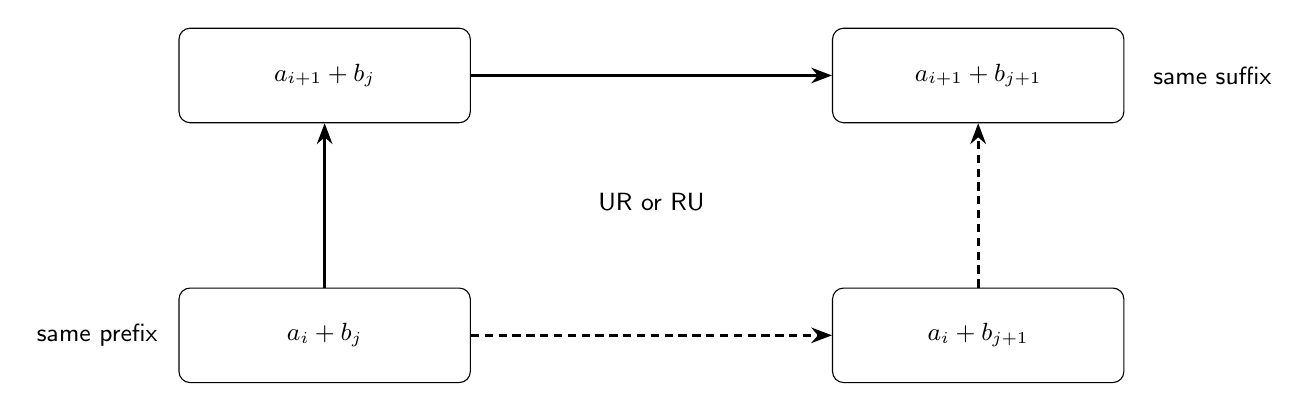
\begin{tikzpicture}[x=1mm,y=1mm,>=Stealth,every node/.style={font=\small}]
\node[draw,rounded corners,minimum width=37mm,minimum height=12mm] (bl) at (0,0) {$a_i+b_j$};
\node[draw,rounded corners,minimum width=37mm,minimum height=12mm] (br) at (83,0) {$a_i+b_{j+1}$};
\node[draw,rounded corners,minimum width=37mm,minimum height=12mm] (tl) at (0,33) {$a_{i+1}+b_j$};
\node[draw,rounded corners,minimum width=37mm,minimum height=12mm] (tr) at (83,33) {$a_{i+1}+b_{j+1}$};
\draw[->,line width=1pt] (bl)--(tl);\draw[->,line width=1pt] (tl)--(tr);
\draw[->,densely dashed,line width=1pt] (bl)--(br);\draw[->,densely dashed,line width=1pt] (br)--(tr);
\node at (41.5,17) {UR or RU};
\node[anchor=east] at (-20,0) {same prefix};
\node[anchor=west] at (104,33) {same suffix};
\end{tikzpicture}
\end{center}

Make two \textbf{full} paths with that same prefix and suffix: one uses up/right, the other right/up in the square. They share $m+n-2$ vertices and hence that many distinct values. Each route's one remaining middle value is different from every shared value because the full route is strictly increasing. Both routes contain the same whole sumset, so after removing shared values the same single value remains:
\[
 a_{i+1}+b_j=a_i+b_{j+1}
 \quad\Longrightarrow\quad
 a_{i+1}-a_i=b_{j+1}-b_j.
\]
This holds for \textbf{every} A gap and \textbf{every} B gap. Fix any B gap: all A gaps equal it. Fix an A gap: all B gaps equal it too. Both inputs have a gap because each has at least two cards. The common gap is positive (strictly increasing inputs) and an integer (integer inputs).

\textbf{Adult prompts if stuck:} ``Can either full path leave a total out at the minimum?'' ``Which values did the two routes share?'' ``What is the one value each has left?'' Do not infer middle equality merely from the routes having equal length; the equality-sized \emph{entire result set} is essential. In the nonminimal demonstration grid, the two alternatives can differ.

\sub{Sufficiency: every index sum occurs}
Write A $=\sset{a+id:0\leq i<m}$ and B $=\sset{b+jd:0\leq j<n}$ with one $d>0$. All totals have the form $a+b+kd$, $0\leq k\leq m+n-2$. Every such $k$ occurs: choose $i=\min(k,m-1)$, $j=k-i$, which keeps $j$ in $0,\ldots,n-1$. The $m+n-1$ totals are distinct because $d>0$. Starts and lengths may differ. A singleton has no gap to compare: page 7 of the student packet supplies the genuine exception.
\newpage

\heading{Return visits, evidence and source scope}
\sub{A theme can support several investigations}
After a first card-design visit, return to the complete fixed-A catalog (5), the gap contrast and singleton (6--7), or the path certificate (8--9). Keep saved trials so returning children resume a question instead of repeating an identical worksheet. The inverse proof (10) is a further mathematical direction; a table need not finish it during its first hour.

Other adult-supported continuations: translate either input and predict what happens to totals and count; enlarge the kit to construct arbitrary-size maxima; compare the common-gap theorem with an irregular fixed A; use signed inputs only after signed-addition readiness and a newly labeled strip (for example $\sset{-2,0,2}+\sset{-3,-1,1}=\sset{-5,-3,-1,1,3}$). Retain the finite-set/no-wrap rules. ``Inverse'' determines structure, not unique starting inputs. Near-minimum counts lead toward deeper inverse problems; no classification of them is claimed here.

\sub{Sources actually consulted; what each supports}
\textbf{Tao and Vu, \emph{Additive Combinatorics}, author-hosted sample:} Prologue Definition 0.1, sample pp.6--7; chapter 2 opening pp.67--69; section 2.1 pp.70--71, Lemma 2.1. These give finite nonempty additive sets, sumset definitions, progression examples, translation and pair-count bounds, and inverse-problem context. Lemma 2.1's general-group lower bound is $\max(|A|,|B|)$, not our sharp integer bound. The sample omits the chapter-5 body. \textbf{The sharp two-set theorem and complete path-swap proof here were independently reconstructed and checked; no uninspected Tao--Vu theorem/page is credited with that proof.}
\href{https://www.math.ucla.edu/~tao/preprints/additive_sample.dvi}{Author sample (math.ucla.edu/\string~tao/preprints/additive\_sample.dvi)}.
The original is kept under \texttt{external-resources/new-themes-52-63/week54-55/}; the converted reading PDF is a temporary research file.

\textbf{Tao, \emph{Sumset and inverse sumset theorems for Shannon entropy}, June 25, 2009:} the Week 55 research record cites its opening/final combinatorial comparison for the $|A+A|\geq2|A|-1$ context. It is not a source for this two-set equality proof; no entropy task is adapted. This guide's primary mathematical consultation was the local book sample, with that post's scope retained from the research record.

\textbf{Givental, Nemirovskaya and Zakharevich, \emph{Math Circle by the Bay}:} Preface pp.viii--ix (PDF pp.9--10), ``How we select our topics'' and ``How we teach,'' were read. They discuss deep themes, independent solving/dialogue, manipulatives and clear child-readable statements. \emph{Our untested inference} is cards and a merged result strip before arrays, with optional depth and readiness gates; the book does not prescribe our kit, table layout or age fit.

\textbf{Stankova and Rike, eds., \emph{A Decade of the Berkeley Math Circle}:} chapter 6, section 3.6 ``The burden of proof,'' pp.113--114 (PDF pp.133--134), was read. Its examples distinguish long strings of verified cases from proof. \emph{Our application} distinguishes successful designs and common-gap conjectures from the universal path argument; we do not use the chapter's induction problems as student tasks.

\textbf{Organizer's year-1 \emph{Handouts 1}:} the unnumbered figurate-number, pictured sum/difference and odd-sum square prompts were read from the original DOCX XML. They provide precedent for visible addition with tiles, not a sumset theorem or evidence that these card procedures worked. Root README and the current context record the value of concreteness/time doing and the later lamp-rule difficulty; the fixed-input partner checks are a new response, not a tested lesson.

All guide wording, tables and the local-square figure are newly authored around established mathematics. The student pages remain the separately revised W55-S-v2 packet. Finite enumeration verifies examples and legal kit designs; the proofs establish arbitrary-size claims. Sources do not validate this adaptation's physical handling, staffing, pacing or classroom understanding. Those pretests and piloting remain unperformed.
\end{document}
